\documentclass[10pt,a4paper]{article}
\usepackage[utf8]{inputenc}
\usepackage[french]{babel}
\usepackage[T1]{fontenc}
\usepackage{amsmath}
\usepackage{amsthm}
\usepackage{amsfonts}
\usepackage{amssymb}
\usepackage{graphicx}
\usepackage{mathrsfs}
\usepackage{color}
\usepackage{url}
\usepackage{hyperref}
\usepackage{cleveref}
\usepackage{listings}
\lstset{
language=R,
basicstyle=\scriptsize\ttfamily,
commentstyle=\ttfamily\color{green},
numbers=left,
numberstyle=\ttfamily\color{black}\footnotesize,
stepnumber=1,
numbersep=5pt,
backgroundcolor=\color{white},
showspaces=false,
showstringspaces=false,
showtabs=false,
frame=single,
tabsize=2,
captionpos=b,
breaklines=true,
breakatwhitespace=false,
keywordstyle=\color{blue},
stringstyle=\color{magenta},
literate=
  {á}{{\'a}}1 {é}{{\'e}}1 {í}{{\'i}}1 {ó}{{\'o}}1 {ú}{{\'u}}1
  {Á}{{\'A}}1 {É}{{\'E}}1 {Í}{{\'I}}1 {Ó}{{\'O}}1 {Ú}{{\'U}}1
  {à}{{\`a}}1 {è}{{\`e}}1 {ì}{{\`i}}1 {ò}{{\`o}}1 {ù}{{\`u}}1
  {À}{{\`A}}1 {È}{{\'E}}1 {Ì}{{\`I}}1 {Ò}{{\`O}}1 {Ù}{{\`U}}1
  {ä}{{\"a}}1 {ë}{{\"e}}1 {ï}{{\"i}}1 {ö}{{\"o}}1 {ü}{{\"u}}1
  {Ä}{{\"A}}1 {Ë}{{\"E}}1 {Ï}{{\"I}}1 {Ö}{{\"O}}1 {Ü}{{\"U}}1
  {â}{{\^a}}1 {ê}{{\^e}}1 {î}{{\^i}}1 {ô}{{\^o}}1 {û}{{\^u}}1
  {Â}{{\^A}}1 {Ê}{{\^E}}1 {Î}{{\^I}}1 {Ô}{{\^O}}1 {Û}{{\^U}}1
  {œ}{{\oe}}1 {Œ}{{\OE}}1 {æ}{{\ae}}1 {Æ}{{\AE}}1 {ß}{{\ss}}1
  {ű}{{\H{u}}}1 {Ű}{{\H{U}}}1 {ő}{{\H{o}}}1 {Ő}{{\H{O}}}1
  {ç}{{\c c}}1 {Ç}{{\c C}}1 {ø}{{\o}}1 {å}{{\r a}}1 {Å}{{\r A}}1
  {€}{{\EUR}}1 {£}{{\pounds}}1
}
\usepackage[french,onelanguage,ruled,lined,linesnumbered]{algorithm2e}
\SetKw{Or}{ou}
\author{\textsc{TRAN Quoc Nhat Han} \& \textsc{Adrien WARTELLE}}
\title{Rapport de projet OS13\\Analyse de politique de maintenance}
\date{\today}
\begin{document}
\maketitle
\renewcommand{\contentsname}{Sommaire}
\tableofcontents
\begin{abstract}
Soient des données liées à la fonctionnement de système, nous déterminons un modèle approprié et puis choisir une politique de maintenance optimal.
\end{abstract}
\section{Maintenance basée sur l'âge}
\subsection{Rappel}
Considérons un système non maintenu. En l'observant, nous obtenons un liste des dates de panne, grâce auquel nous construirerons une politique de remplacement systématique basée sur l'âge : \emph{Nous remplaçons lorsque le système tombe en panne ou qu'il survit une durée $t_0$}.

Le but est de minimiser le coût moyen cumulé.
\begin{equation}
    \label{coutmoyduree}
    \mathbb{E}(C) = \frac{\mathbb{E}(C(S))}{\mathbb{E}(S)}
\end{equation}

Où $S$ est la variable aléatoire représentant la date de remplacement et $C(S)$ est le coût de maintenance cumulé à l'instant $S$ (sachant que $C(S)$ est $c_c (=1200)$ si une maintenance corrective et $c_p(=800)$ si préventive).
\subsection{Modéliser la durée de vie du système}
L'importation de données de \texttt{FailureTimes\_5.csv} (l'annexe \ref{annexe:import_pannes}) expose les dates de pannes de l'ordre grandement variée ($300$ à $27000$) (l'annexe \ref{annexe:premier_histo}). 

Exponentiel des valeurs extrèmes résulteront $Inf$, ce qui est indésirable. Alors nous devons forcément les réduire en les divisant par un scalaire \texttt{scale}, prenons par example $1000$.  (Figure \ref{histo1})
\begin{figure}[!htb]
    \centering
    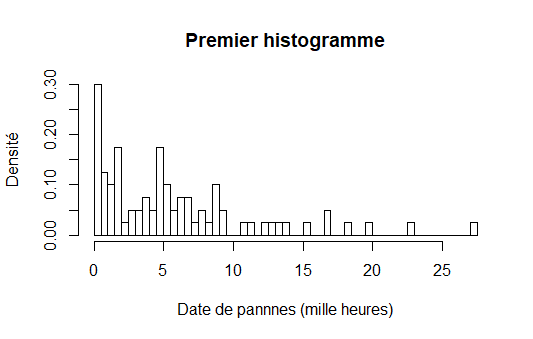
\includegraphics[width=\textwidth]{img/premier_histo.png}
    \caption{Le premier histogramme de distribution de pannes}
    \label{histo1}
\end{figure}

Les pannes se concentrent autour de 2 sommets, l'un à $[0; 0,5]$ et l'autre à $[4,5; 5]$. Ceci nous fait penser naturellement à un mixage de deux lois.

Nous pouvons remarquer que les valeurs sont positives (étant données que ce sont des temps) et que la
distribution semble posséder deux parties importantes. Une dont le sommet se situe près de zéro et qui est suivi d'une pente forte, et l'autre sommet est à une valeur non nulle (5) que la distribution locale en forme de pic.
Nous avons donc penser estimer un mixage de loi \emph{Exponentielle} et \emph{Gamma} afin de modéliser
les données. En effet la première partie correspondrait à une loi exponentielle tandis que la seconde à
une loi gamma (Et .

La fonction de densité avec le paramètre $\theta  = \left( {p_1, p_2, \lambda ,\alpha ,\beta } \right)$ :
\begin{align}
    \begin{split}
        \label{fMelExpGam}
        {f_\theta }\left( x \right) & = {p_1}{f_1}\left( x \right) + {p_2}{f_2}\left( x \right) \\
        & = {p_1}\lambda {e^{ - \lambda x}} + {p_2}\frac{{{\beta ^\alpha }}}{{\Gamma \left( \alpha  \right)}}{x^{\alpha  - 1}}{e^{ - \beta x}}
    \end{split}
\end{align}

Où $f_1, f_2$ désignent réspectivement $exp(\lambda)$ et $\Gamma(\alpha, \beta)$; $p_1, p_2 > 0: p_1 + p_2 = 1$.

Nous allons utiliser l'algorithme EM, la méthode la plus efficace pour estimer le MLE de mixage fini.

Soit $X$ la variable aléatoire de durée de vie du système. Soient $\left( {{x_1},...,{x_N}} \right)$ les observations.

Soit la matrice de probabilité d'appartenance $(\zeta_{ki})$ : $\zeta_{ki}$ vaut la probabilité que $x_i$ suive la loi $f_k$.
\begin{equation}
    \label{zeta}
    {\zeta _{ki}} = \frac{{{p_k}{f_k}\left( {{x_i}} \right)}}{{{p_1}{f_1}\left( {{x_i}} \right) + {p_2}{f_2}\left( {{x_i}} \right)}}\forall k = \overline {1,2} \forall i = \overline {1,N}
\end{equation}

La fonction de vraisemblance : 
\begin{equation}
    \label{funlik}
    \ln \Lambda  = \sum\limits_{i = 1}^N {\ln {f_\theta }\left( {{x_i}} \right)}  = \sum\limits_{i = 1}^N {\ln \left( {{p_1}{f_1}\left( {{x_i}} \right) + {p_2}{f_2}\left( {{x_i}} \right)} \right)}
\end{equation}

Nous cherchons à maximiser $\ln \Lambda$ en la dérivant selon $\lambda, \alpha, \beta$.

Pour $\lambda$ :
\begin{align}
    \frac{\partial }{{\partial \lambda }}\ln \Lambda  & = \sum\limits_{i = 1}^N {\frac{{{p_1}{e^{ - \lambda {x_i}}} - {p_1}\lambda {x_i}{e^{ - \lambda {x_i}}}}}{{{p_1}{f_1}\left( {{x_i}} \right) + {p_2}{f_2}\left( {{x_i}} \right)}}} \nonumber \\
    & = \sum\limits_{i = 1}^N {\frac{{{p_1}{f_1}\left( {{x_i}} \right)}}{{{p_1}{f_1}\left( {{x_i}} \right) + {p_2}{f_2}\left( {{x_i}} \right)}}\left( {\frac{1}{\lambda } - {x_i}} \right)} \nonumber  \\
    & = \frac{1}{\lambda }\sum\limits_{i = 1}^N {{\zeta _{1i}}}  - \sum\limits_{i = 1}^N {{\zeta _{1i}}{x_i}}  = 0 \nonumber \\
    \label{lambda}
    \Leftrightarrow \lambda  & = \frac{{\sum\limits_{i = 1}^N {{\zeta _{1i}}} }}{{\sum\limits_{i = 1}^N {{\zeta _{1i}}{x_i}} }}
\end{align}

Pour $\beta$ :
\begin{align}
    \frac{\partial }{{\partial \beta }}\ln \Lambda  & = \sum\limits_{i = 1}^N {\frac{{{p_2}x_i^{\alpha  - 1}}}{{\Gamma \left( \alpha  \right)}}\frac{{\alpha {\beta ^{\alpha  - 1}}{e^{ - \beta {x_i}}} - {\beta ^\alpha }{x_i}{e^{ - \beta {x_i}}}}}{{{p_1}{f_1}\left( {{x_i}} \right) + {p_2}{f_2}\left( {{x_i}} \right)}}} \nonumber \\
    & = \sum\limits_{i = 1}^N {\frac{{{p_2}{f_2}\left( {{x_i}} \right)}}{{{p_1}{f_1}\left( {{x_i}} \right) + {p_2}{f_2}\left( {{x_i}} \right)}}\left( {\frac{\alpha }{\beta } - {x_i}} \right)} \nonumber \nonumber \\
    & = \frac{\alpha }{\beta }\sum\limits_{i = 1}^N {{\zeta _{2i}}}  - \sum\limits_{i = 1}^N {{\zeta _{2i}}{x_i}}  = 0 \nonumber \\
    \label{beta}
    \Leftrightarrow \beta & = \alpha \frac{{\sum\limits_{i = 1}^N {{\zeta _{2i}}} }}{{\sum\limits_{i = 1}^N {{\zeta _{2i}}{x_i}} }}
\end{align}

Pour $\alpha$ : 
\begin{align*}
    \frac{\partial }{{\partial \alpha }}\ln \Lambda  & = \sum\limits_{i = 1}^N {\frac{{{p_2}{e^{ - \beta {x_i}}}}}{{{p_1}{f_1}\left( x \right) + {p_2}{f_2}\left( x \right)}}\left( {\frac{{\beta \left( {\ln \beta  + \ln {x_i}} \right){{\left( {\beta {x_i}} \right)}^{\alpha  - 1}}}}{{\Gamma \left( \alpha  \right)}} - {\beta ^\alpha }{x^{\alpha  - 1}}\frac{{\Psi \left( \alpha  \right)}}{{\Gamma \left( \alpha  \right)}}} \right)} \\
    & = \sum\limits_{i = 1}^N {\frac{{{p_2}{f_2}\left( {{x_i}} \right)}}{{{p_1}{f_1}\left( x \right) + {p_2}{f_2}\left( x \right)}}\left( {\ln \beta  + \ln {x_i} - \Psi \left( \alpha  \right)} \right)} \\
    & = \left( {\sum\limits_{i = 1}^N {{\zeta _{2i}}} } \right)\ln \beta  + \sum\limits_{i = 1}^N {{\zeta _{2i}}\ln {x_i}}  - \Psi \left( \alpha  \right)\left( {\sum\limits_{i = 1}^N {{\zeta _{2i}}} } \right) = 0 \\
    \Leftrightarrow 0 & = \ln \alpha  + \ln \frac{{\sum\limits_{i = 1}^N {{\zeta _{2i}}} }}{{\sum\limits_{i = 1}^N {{\zeta _{2i}}{x_i}} }} + \frac{{\sum\limits_{i = 1}^N {{\zeta _{2i}}\ln {x_i}} }}{{\sum\limits_{i = 1}^N {{\zeta _{2i}}} }} - \Psi \left( \alpha  \right) \text{ (substitué par \eqref{beta})} \\
    \Leftrightarrow 0 & = \ln \alpha  - \Psi \left( \alpha  \right) - c
\end{align*}

Où $c = \ln \left( {\frac{{\sum\limits_{i = 1}^N {{\zeta _{2i}}{x_i}} }}{{\sum\limits_{i = 1}^N {{\zeta _{2i}}} }}} \right) - \frac{{\sum\limits_{i = 1}^N {{\zeta _{2i}}\ln \left( {{x_i}} \right)} }}{{\sum\limits_{i = 1}^N {{\zeta _{2i}}} }}$; $\Psi$ est la fonction digamma.

Selon la méthode de Newton-Rashphon, nous pouvons résoudre $\alpha$ numériquement avec ce formul itératif :
\[{\alpha _{r + 1}} = {\alpha _r} - \frac{{\ln {\alpha _r} + \Psi \left( {{\alpha _r}} \right) - c}}{{\frac{1}{{{\alpha _r}}} - \Psi '\left( {{\alpha _r}} \right)}}\]

\cite{bib:gamma} propose un autre formule convergeant plus vite :
\begin{equation}
    \label{alpha}
    \frac{1}{{{\alpha _{r + 1}}}} = \frac{1}{{{\alpha _r}}} + \frac{{\ln \left( {{\alpha _r}} \right) - \Psi \left( {{\alpha _r}} \right) - c}}{{\alpha_r^2\left( {\frac{1}{{{\alpha _r}}} - \Psi '\left( {{\alpha _r}} \right)} \right)}}
\end{equation}

Avec $\Psi'$ la fonction trigamma. L'itération part avec ${\alpha _0} = \frac{{0.5}}{c}$.

Au final, pour $p_k$:
\begin{equation}
    \label{p}
    {p_k} = \frac{{\sum\limits_{i = 1}^N {{\zeta _{ki}}} }}{N}\forall k = \overline {1,2}
\end{equation}

Etant donné \eqref{zeta}, \eqref{lambda}, \eqref{beta}, \eqref{alpha} et \eqref{p}, nous définissons l'algorithme EM :
\begin{enumerate}
    \item \textbf{Initialisation :} Choisir $\theta_{0}$.
    \item \textbf{Etape E :} Evaluer $(\zeta_{ki})$ sachant $\theta_{c}$ en utilisant \eqref{zeta}.
    \item \textbf{Etape M :} Calculer $\theta_{c+1}$ à l'aide des équations \eqref{lambda}, \eqref{beta}, \eqref{alpha} et \eqref{p}. \\
    \emph{Note :} Pour $\alpha$, l'itération se termine quand $\left| {{\alpha _{r + 1}} - {\alpha _r}} \right| < {\varepsilon_\alpha }$ où $\varepsilon_\alpha$ est un réel positif fixé à l'initialisation.
    \item \textbf{Evaluation :} Si $\left\| {{\theta_{c + 1}} - {\theta_c}} \right\| < {\varepsilon _\theta }$ ($\varepsilon_\theta$ est un réel positif fixé à l'initialisation), l'algorithme s'arrête et $\theta = \theta_{vieux}$. \\ Sinon, reviens à l'étape E avec $\theta_{vieux} \leftarrow \theta_{nouveau}$.
\end{enumerate}

Avant de lancer l'algorithme nous essayons d'obtenir un ensemble de paramètres initiaux $\theta_{0}$
qui soient cohérent avec la distribution des données. Nous avons choisi 
\[\left( {{p_{1_0}},{p_{2_0}},\lambda_{0} ,\alpha_{0} ,\beta_{0} } \right) = \left( {0.5;0.5;1;10;2} \right)\]

\begin{figure}[!hbt]
    \centering
    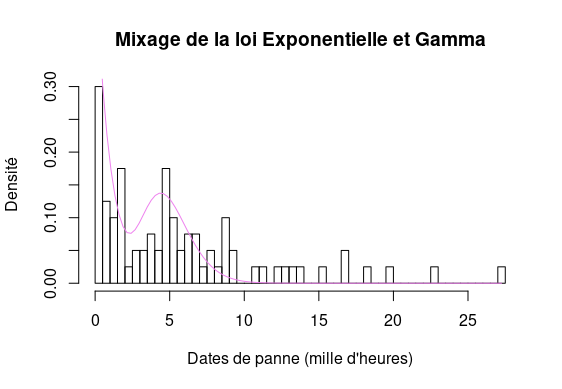
\includegraphics[width=\textwidth]{img/loi_initiale_Exp_Gamma.png}
    \caption{Mixage de la loi Exponentielle et Gamma : paramètres initiaux}
    \label{mixage_init}
\end{figure}

Après l'utilisation de l'algorithme EM, nous avons obtenu le résultat :
\[\left( {{p_1},{p_2},\lambda ,\alpha ,\beta } \right) = \left( {0.2194518;0.7805482;1.56738;1.665659;0.2332427} \right)\]

D'où nous traçons la fonction de densité $f_\theta$ trouvé (figure \ref{mixage}) et réalisons un test de Kolmogorov-Smirnov qui donne $p-value=0,9663111$ signifiant $96,63\%$ de nous tromper si nous rejetons ce modèle. Nous l'acceptons alors, quoiqu'il ne génère pas 2 sommets comme la remarque initiale. Le code est trouvable à l'annexe \ref{annexe:em_exp_gamma}.

\begin{figure}[!hbt]
    \centering
    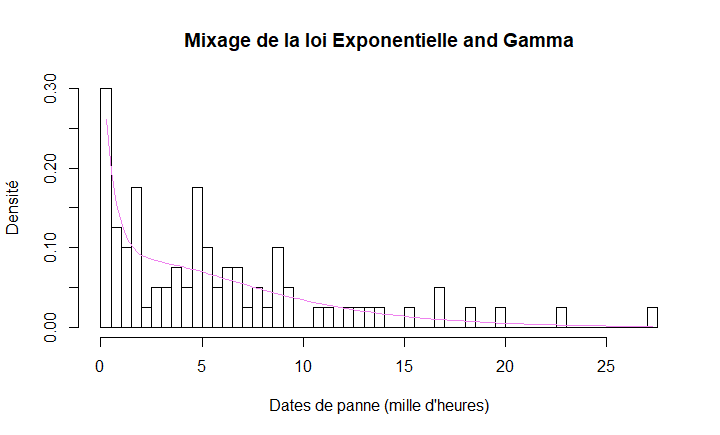
\includegraphics[width=\textwidth]{img/EM_Exp_Gamma.png}
    \caption{Mixage de la loi Exponentielle et Gamma : paramètres finaux}
    \label{mixage}
\end{figure}

\subsection{La politique de maintenance basée sur l'âge}

Avec la fonction $f_\theta$ trouvée, nous construirerons la politique optimale.

Nous avons par définition : $S = \min \left( {X,{t_0}} \right)$.

Autrement dit, $S = X{\mathbb{I}_{\left\{ {X < {t_0}} \right\}}} + {t_0}{\mathbb{I}_{\left\{ {X \geqslant {t_0}} \right\}}}$.

Traduit au coût : $C\left( S \right) = {C_c}{\mathbb{I}_{\left\{ {X < {t_0}} \right\}}} + {C_p}{\mathbb{I}_{\left\{ {X \geqslant {t_0}} \right\}}}$, avec $C_c, C_p$ les coûts de maintenances correctives et préventives réspectivement.

Le coût moyen :
\begin{align}
    \label{coutmoy}
    \mathbb{E}\left( {C\left( S \right)} \right) & = {c_c}\mathbb{E}\left( {{\mathbb{I}_{\left\{ {X < {t_0}} \right\}}}} \right) + {c_p}\mathbb{E}\left( {{\mathbb{I}_{\left\{ {X \geqslant {t_0}} \right\}}}} \right) \nonumber \\
    & = {c_c}P\left( {X < {t_0}} \right) + {c_p}P\left( {X \geqslant {t_0}} \right) \nonumber \\
    & = {c_c}{F_\theta }\left( {{t_0}} \right) + {c_p}\left( {1 - {F_\theta }\left( {{t_0}} \right)} \right) \nonumber \\
    & = \left( {{c_c} - {c_p}} \right){F_\theta }\left( {{t_0}} \right) + {c_p}
\end{align}

La durée moyenne :
\begin{align}
    \label{dureemoy}
    \mathbb{E}\left( S \right) & = \mathbb{E}\left( {X{\mathbb{I}_{\left\{ {X < {t_0}} \right\}}}} \right) + {t_0}\mathbb{E}\left( {{\mathbb{I}_{\left\{ {X \geqslant {t_0}} \right\}}}} \right)\nonumber\\
    & = \int_0^{{t_0}} {x{f_\theta }\left( x \right)dx}  + {t_0}P\left( {X \geqslant {t_0}} \right) \nonumber \\
    & = x{F_\theta }\left( x \right)|_0^{{t_0}} - \int_0^{{t_0}} {{F_\theta }\left( x \right)dx}  + {t_0}\left( {1 - {F_\theta }\left( {{t_0}} \right)} \right) \nonumber \\
    & = {t_0} - \int_0^{{t_0}} {{F_\theta }\left( x \right)dx}
\end{align}

De \eqref{coutmoy} et \eqref{dureemoy}, nous détaillons le coût moyen sur une durée de temps \eqref{coutmoyduree} :
\begin{equation}
    \label{coutmoydureedet}
    \mathbb{E}\left( C \right) = \frac{{\mathbb{E}\left( {C\left( S \right)} \right)}}{{\mathbb{E}\left( S \right)}} = \frac{{\left( {{c_c} - {c_p}} \right){F_\theta }\left( {{t_0}} \right) + {c_p}}}{{{t_0} - \int_0^{{t_0}} {{F_\theta }\left( x \right)dx} }}
\end{equation}

L'annexe \eqref{annexe:optim_e_c} montrer comment chercher l'optimum numériquement. La valeur minimum est $t_0 = 27,29639$ (mille heures), correspondant à un coût moyen de $210,6402$. Nous constatons que $t_0^{min}$ est très proche du maximum de durée de vie, indiquant que l'optimisation de $t_0$ est inutile car le système ne viellit pas.

\section{Maintenance basée sur dégradation}
\subsection{Rappel}
En observant multiples systèmes identiques, nous effectuons des mesures de dégradation sur des intervalles de temps réguliers tout au long de leurs durée de vie.

La valeur limite de dégradation est $L=20$. C'est-à-dire lorsque le niveau de dégradation dépasse $L$, le système tombe en panne et nous ne pourrons plus le mesurer.

On souhaite de mettre en place une politique de maintenance conditionnelle, basée sur un seuil $M$ inférieur à $L$ et l'intervalle de temps $\Delta T$ entre les inspections répétive. Appellons $X_t$ le niveau de dégradation à l'instant $t$ (instant d'une inspection).
\begin{itemize}
    \item Si $X_t < M$, nous laissons le système tel quel.
    \item Si $M \leq X_t < L$, un remplacement préventif est réalisé au coût $c_p$. Et puis $X_t$ est remis à $0$.
    \item Si $X_t \geq L$, un remplacement correctif est fait au coût $c_c$. Et puis $X_t$ est remis à $0$.
\end{itemize}

Le but est minimiser le coût moyen sur une durée de temps \eqref{coutmoyduree} en bien choissisant le seuil $M$ et l'intervalle d'inspection $\Delta T$.
\subsection{Modéliser la dégradation du système}

Soient les données de \texttt{DegradLevel\_2.csv}, nous traçons leurs processus de dégrader (figure \eqref{fig:trace_degrad}). (Les annexes \eqref{annexe:import_degrad} et \eqref{annexe:premier_plot_degrad})

Comme les temps d'inspection sont de l'ordre millier, il vaudrait de les diviser par un scalaire (par example, $scale = 1000$) afin d'assurer la précision de calcul numérique.

\begin{figure}
    \centering
    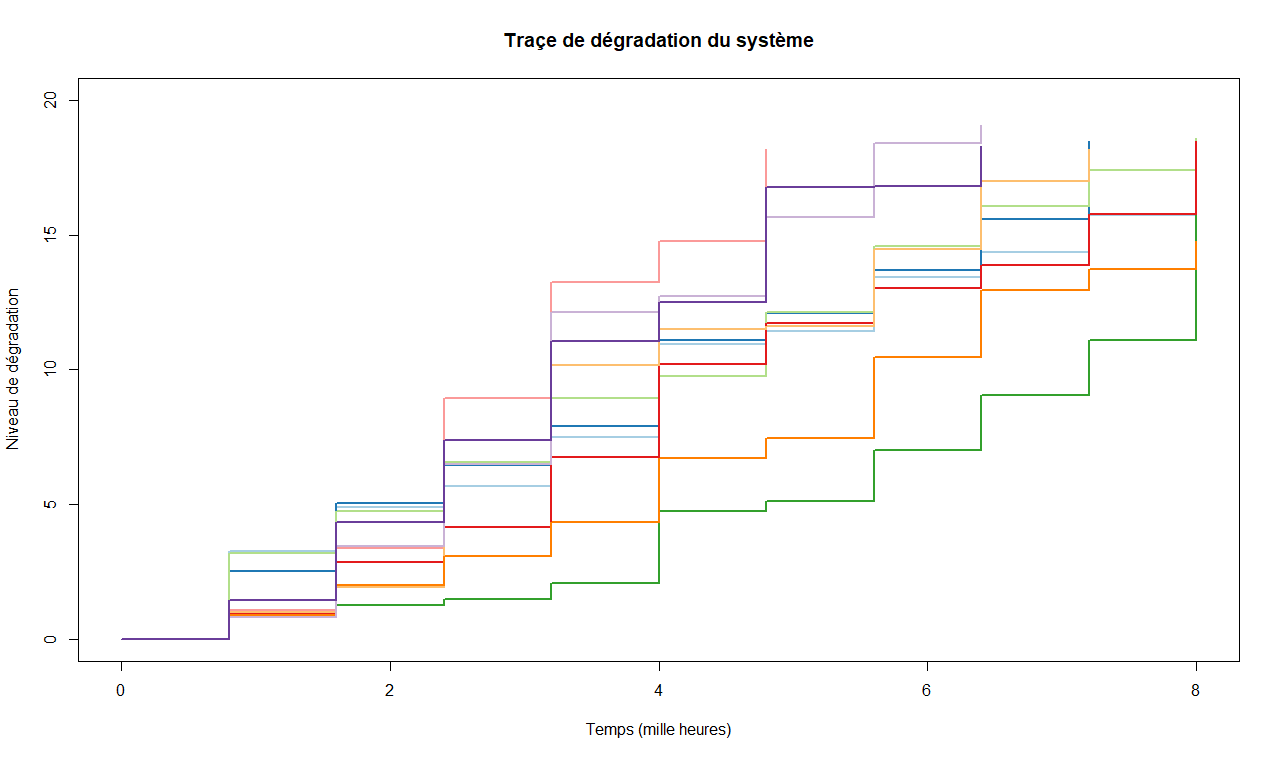
\includegraphics[width=\textwidth]{img/trace_degrad.png}
    \label{fig:trace_degrad}
\end{figure}

Nous voyons les accroissements positifs, suggérant un modèle de processus Gamma.

Soit $X(t)$ la variable aléatoire de dégradation du système. Supposons que $X(t) - X(s) \sim \Gamma(a(t-s),b)\,\forall t > s > 0$. Nous allons estimer les paramètres $a,b$ en modélisant la distribution des incréments entre deux moments successifs.

Fixons $t-s = \delta = 0.8$, car les mesures donnés sont effectués au bout de chaque intervalle de $0.8$.

L'histogramme des incréments :
\begin{figure}[!h]
    \centering
    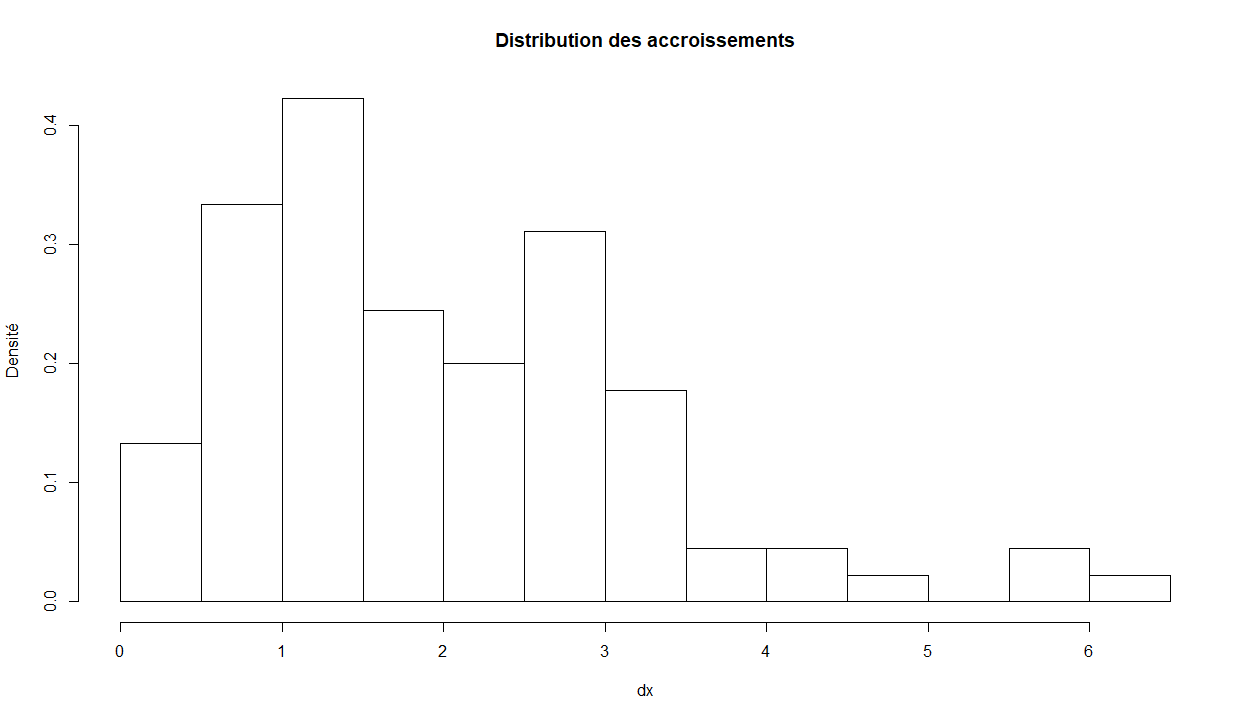
\includegraphics[width=\textwidth]{img/histo_degrad.png}
    \caption{Histogramme des incréments de l'intervalle $\delta = 0.8$}
    \label{fig:histo_degrad}
\end{figure}

A l'aide du librairie MASS : $\left( {a;b} \right) = \left( {\frac{\alpha }{\delta };\beta } \right) = \left( {2.843101;1.140354} \right)$ où $(\alpha, \beta)$ sont les paramètres estimés par MASS. Le code est mis à l'annexe \eqref{annexe:estim_degrad}.

Un test rapide de Kolmogorov-Smirnov nous donne $p-value = 0.8651934$, indiquant le modèle est acceptable.
\begin{figure}[!h]
    \centering
    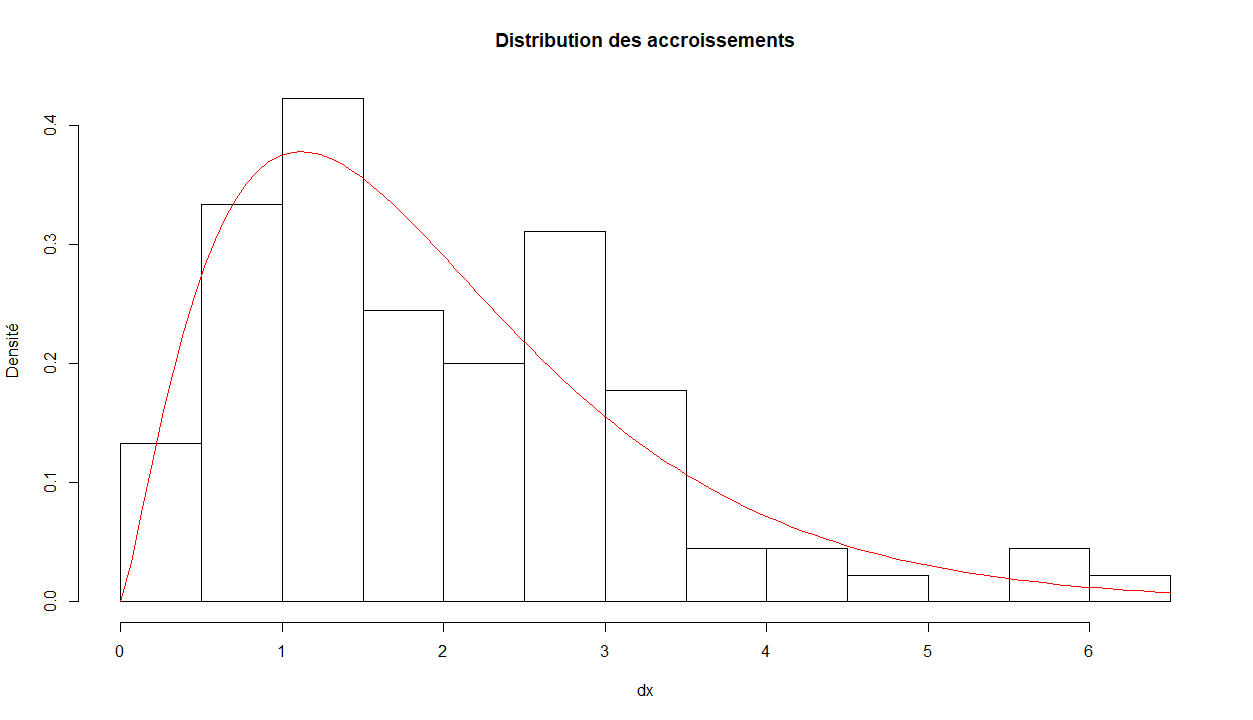
\includegraphics[width=\textwidth]{img/histo_dens_degrad.png}
    \caption{Histogramme et la courbe de densité estimé des incréments de l'intervalle $\delta = 0.8$}
    \label{fig:histo_dens_degrad}
\end{figure}

D'autant plus, si nous refaisons les calculs ci-dessus avec $\delta = 1.6, 2.4, 3.2, etc.$, nous voyons les valeurs de $a$ et $b$ ne varient pas trop. Alors, nous choisissons le couple $(a,b)$ avec $p$ le plus grand. ($\delta$ trop grand réduira nombreux de données, résultant une perte importante de précision)

\begin{figure}[!h]
    \centering
    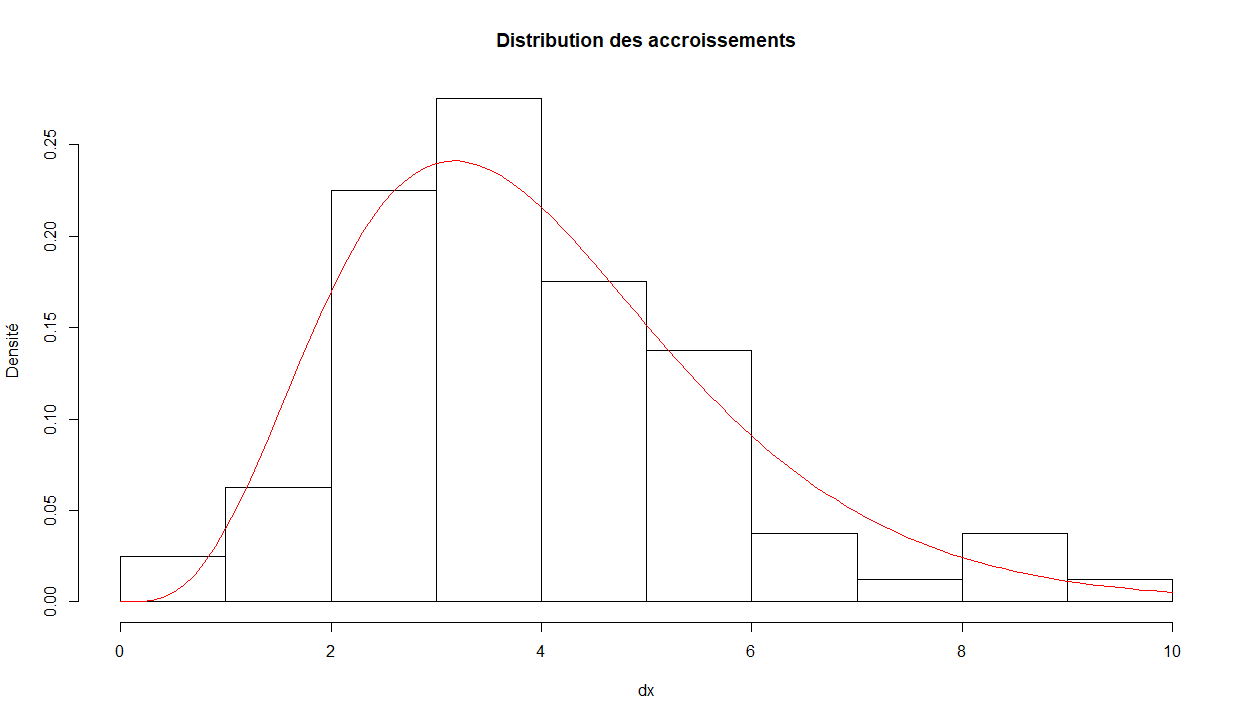
\includegraphics[width=\textwidth]{img/histo_dens_degrad_1_6.png}
    \caption{Histogramme et la courbe de densité estimé des incréments de l'intervalle $\delta = 1.6$}
    \label{fig:histo_dens_degrad_1_6}
\end{figure}

\begin{table}[!h]
    \centering
    \begin{tabular}{|c|c|c|c|}
        \hline
        $\delta$ & $a$ & $b$ & $p$ \\
        \hline
        0.8 & 2.8431009 & 1.1403540 & 0.8651934\\
        1.6 & 3.0207719 & 1.2091646 & 0.9919939\\
        2.4 & 3.0187497 & 1.1907719 & 0.1279252\\
        3.2 & 2.997763 & 1.185547 & 0.300610\\
        4.0 & 3.5036580 & 1.4061063 & 0.6307951\\
        \hline
    \end{tabular}
    \caption{Calcul $(a,b)$ avec différents $\delta$}
\end{table}

Au final, $X(t) - X(s) \sim \Gamma(a(t-s),b) \forall t > s > 0$ avec $$(a,b) = (3.0207719;1.2091646)$$

\subsection{La politique de maintenance basée sur dégradation}

Cette politique, outre que $c_c=1200$ et $c_p=800$, introduit ainsi le coût d'inspection répétive $c_i = 10$.

Soit $S$ la variable aléatoire représentant la date de remplacement; $C(S)$ est le coût de maintenance cumulé à l’instant $S$, et $N(S)$ le nombre d'inspections depuis la dernière remplacement jusqu'à $S$.

\begin{equation}
    \label{c_s_de}
    C\left( S \right) = {c_i}N\left( S \right) + {c_p}{\mathbb{I}_{\left\{ {L > {X_{N\left( S \right)}} \geq M} \right\}}} + {c_c}{\mathbb{I}_{\left\{ {{X_{N\left( S \right)}} \geq L} \right\}}}
\end{equation}

Posons ${F_t} = \Gamma \left( {at,b} \right)$ et les instants d'inspections ${t_1},{t_2},...,{t_{N\left( S \right)}}$ avec ${t_{j + 1}} - {t_j} = \Delta T$. Puisque $t_0 = 0$, nous aurons ${t_k} = k\Delta T$ et $X_{t_k} \sim F_{k\Delta T}$.

Comme le calcul analytique de $C(S)$ et $N(S)$ devient grossier, nous passons à la méthode Monté Carlo, qui nous permet d'estimer la vraie valeur en répéter un nombre suffisant de simulations.

\begin{algorithm}[!h]
    \caption{Mesurer la durée de vie d'un processus}
    \label{algo:s}
    \KwIn{$p$ le processus\newline
        $\Delta T$ l'intervalle d'inspection\newline
        $M$ le seuil de maintenance préventive
    }
    \KwOut{$S$ la durée de vie}
    $len \leftarrow $ longeur de $p$\;
    \eIf{$p_{len} < M$}{
        \tcp{La simulation n'est pas suffisante longue}
        \Return{0}
    }{
        $n_s \leftarrow$ le dernier index de $p$ tel que $p_{n_s} < M$\;
        \Return{$n_s + 1$}
    }
\end{algorithm}

\begin{algorithm}[!h]
    \caption{Mesurer le coût de maintenance d'un processus}
    \label{algo:c_s}
    \KwIn{$p$ le processus\newline
    $M$ le seuil
    }
    \KwOut{$C(S)$ le coût de maintenance}
    $cout \leftarrow 0$\;
    $len \leftarrow $ longeur de $p$\;
    \If{$p_{len} \geq M$}{
        $n_s \leftarrow$ le dernier index de $p$ tel que $p_{n_s} < M$\;
        \tcp{$n_s$ correspond le nombre d'inspection}
        $cout \leftarrow cout + c_i * n_s$\;
        \tcp{A l'inspection suivante}
        \eIf{$p_{n_s + 1} \geq L$}{
            \tcp{Le système est tombé en panne}
            $cout \leftarrow cout + c_c$\;
        }{
            \tcp{Le système fonctionne encore}
            $cout \leftarrow cout + c_p$\;
        }
    }
    \tcp{Le coût est zéro si le niveau de dégradation ne dépasse pas encore $M$}
    \Return{$cout$}
\end{algorithm}

\begin{algorithm}[!h]
    \caption{Simuler le processus et calculer $\widehat{\mathbb{E}(C)}$}
    \label{algo:e_c}
    \KwIn{$\Delta T$ l'intervalle d'inspection\newline
    $M$ le seuil\newline
    $nSim$ le nombre de simulation\newline
    $nStep$ le nombre d'inspection maximale}
    \KwOut{$\widehat{\mathbb{E}(C)}$ la valeur approximative}
    Générer la matrice de l'incréments $simStep$ de taille $nSim \times nStep$ aux valeurs aléatoires selon la loi $\Gamma(a\Delta T, b)$\;
    Calculer la matrice de processus $simProc$ de taille $nSim \times nStep$ en faisant la somme cumulative de $simStep$ horizontallement\;
    $simTime \leftarrow$ les durées de vie de processus en appliquant l'algorithme \eqref{algo:s}\;
    $simCost \leftarrow$ les coûts de processus en appliquant l'algorithme \eqref{algo:c_s}\;
    $meanSimCost \leftarrow$ la moyenne de tous les coûts non nuls de $simCost$\;
    $meanSimTime \leftarrow$ la moyenne de durée de vie non nuls de $simTime$\;
    $meanCostTime \leftarrow \frac{meanSimCost}{meanSimTime}$\;
    \If{$meanSimCost$ est \texttt{NaN} \Or $meanSimTime$ est \texttt{NaN}}{
        $meanCostTime \leftarrow MAX\_DOUBLE$\;
    }
    \Return{$meanCostTime$}
\end{algorithm}

Puisque l'algorithme \eqref{algo:e_c} utilise de calcul matricielle pour accélérer la traitement, $nStep$ doit être fixé judicieusement pour qu'on aura pas "trop" de simulations où $X_{t_{nStep}} < M$ (ce qui va forcer les valeurs de $C(S)$ et $S$ à zéro selon les algorithmes \eqref{algo:s} et \eqref{algo:c_s}). Soit $\alpha$ la probabilité de cet événement.

\begin{align*}
    P\left( {{X_{{t_{nStep}}}} < M} \right) & = \alpha  \\
    \Leftrightarrow {F_{nStep*\Delta T}}\left( M \right) & = \alpha \\
    \Leftrightarrow \Gamma \left( {a*nStep*\Delta T,b} \right)\left( M \right) & = \alpha 
\end{align*}

Nous testons quelques valeurs de $F$. Comme $F$ est croissant, nous l'évaluons directement à $M=20$.

\begin{table}[!h]
    \centering
    \begin{tabular}{|c|c|}
      \hline
      $nStep * \Delta T$ &  $\Gamma \left( {a*nStep*\Delta T,b} \right)\left( 20 \right)$\\
      \hline
      8 & 0.5284405 \\
      10 & 0.1319799 \\
      12 & 0.01300913 \\
      13 & 0.002925565 \\
      14 & 0.000533971 \\
      \hline
    \end{tabular}
    \caption{Estimation de $nStep * \Delta T$}
    \label{tab:nstep}
\end{table}

La fonction distribution décroît selon $nStep*\Delta T$. Et pourtant, $\alpha \leq 1\%$ nous suffit. Et plus grand $nStep$, plus lente la traitement. C'est pourquoi, basé sur la table \eqref{tab:nstep}, nous emploirons
\[nStep = \left\lfloor {\frac{{13}}{{\Delta T}}} \right\rfloor \]

\begin{algorithm}[!h]
    \caption{Optimiser la politique de maintenance basée sur dégradation}
    \label{algo:optim_degrad}
    \KwIn{$[L_{\Delta T}, U_{\Delta T}]$ l'intervalle de recherche de $\Delta T$\newline
        $[L_{M}, U_{M}]$ l'intervalle de recherche de $M$\newline
        $\tau$ la tolérance\newline
        $d_{\Delta T}$ le nombre de points à évaluer pour $\Delta T$\newline
        $d_M$ le nombre de points à évaluer pour $M$\newline
        $e_{\Delta T}$ le ratio de réduction sur l'intervalle de $\Delta T$\newline
        $e_M$ le ratio de réduction sur l'intervalle de $M$
    }
    \KwOut{$\Delta T^*$ l'intervalle d'inspection optimal\newline
        $M^*$ le seuil optimal\newline
        $o^*$ la valeur objective optimale
    }
    \tcp{Suivre le principe de diachotomie}
    $\Delta T^* \leftarrow 0$\;
    $M^* \leftarrow 0$\;
    $o^* \leftarrow 0$\;
    \While{${\left( {\frac{{{L_{\Delta T}} - {U_{\Delta T}}}}{{{d_{\Delta T}}}}} \right)^2} + {\left( {\frac{{{L_M} - {U_M}}}{{{d_M}}}} \right)^2} \geqslant \tau^2 $}{
        \tcp{Evaluer}
        $I_{\Delta T} \leftarrow$ l'ensemble de $d_{\Delta T}$ points égaux-distances de $[L_{\Delta T}, U_{\Delta T}]$\;
        $I_{M} \leftarrow$ l'ensemble de $d_{M}$ points égaux-distances de $[L_{M}, U_{M}]$\;
        $Z \leftarrow $ résultats d'appliquer l'algorithme \eqref{algo:e_c} pour chaque point sur la grille $I_{\Delta T} \times I_M$\;
        \tcp{Chercher le minimum}
        $(i^*,j^*) \leftarrow $ l'indice de premier minimum de $Z$\;
        $\Delta T^* \leftarrow $ l'élément $i^*$-ième de $I_{\Delta T}$\;
        $M^* \leftarrow $ l'élément $j^*$-ième de $I_{M}$\;
        $o^* \leftarrow Z_{i^*,j^*}$\;
        \tcp{Ajuster la nouveau zone de recherche autour du minimum actuel}
        ${l_{\Delta T}} \leftarrow {L_{\Delta T}} - {U_{\Delta T}}$\;
        ${l_M} \leftarrow {L_M} - {U_M}$\;
        ${L_{\Delta T}} \leftarrow \min \left( {\Delta {T^*} + \frac{{{l_{\Delta T}}}}{{{d_{\Delta T}}}},{L_{\Delta T}}} \right)$\;
        ${U_{\Delta T}} \leftarrow \max \left( {\Delta {T^*} - \frac{{{l_{\Delta T}}}}{{{d_{\Delta T}}}},{U_{\Delta T}}} \right)$\;
        ${L_M} \leftarrow \min \left( {{M^*} + \frac{{{l_M}}}{{{d_M}}},{L_M}} \right)$\;
        ${U_M} \leftarrow \max \left( {{M^*} - \frac{{{l_M}}}{{{d_M}}},{U_M}} \right)$\;
    }
    \Return{$(\Delta T^*, M^*, o^*)$}
\end{algorithm}

Le code implémenté se situe à l'annexe \ref{annexe:optim_degrad}. 

Bien que le résultat n'est pas stable, nous pouvons arriver à une valeur approximative après plusieurs fois d'appliquer l'algorithme \ref{algo:optim_degrad} sur l'intervalle $[0.001, 4] \times [0, 20]$ : 
\begin{align*}
    (\Delta T^*, M^*, o^*) = (& 0.001007627 \text{ (mille heures)},\\
    & 18.58027,\\
    & 10.10541 \text{ (euros/mille heures)})
\end{align*}

Ce résultat nous semble logique car :
\begin{itemize}
    \item $\Delta T^*$ faible (grâce à $c_i$ pas cher) nous permet d'observer mieux et just à temps le système.
    \item $M^*$ pas trop loin de $L$ va remplacer la plupart de $c_c$ par $c_p$ pour économiser.
\end{itemize}

\begin{figure}
    \centering
    \caption{Représentation graphique de $E(C)$}
    \label{fig:e_c}
    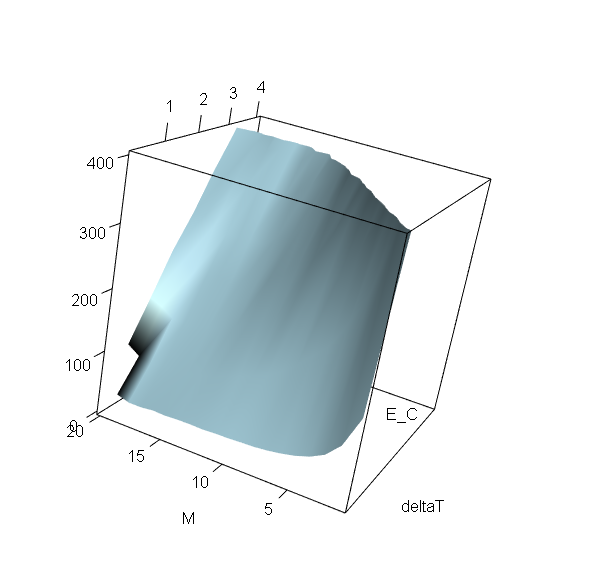
\includegraphics[width=0.8\textwidth]{img/E_C_degrad.png}
\end{figure}

\clearpage
\section{Annexe}
\subsection{L'importation de données de pannes}
\label{annexe:import_pannes}
\lstinputlisting[language=R]{part1/import_failures.R}
\subsection{Le premier histogramme de distribution de pannes}
\label{annexe:premier_histo}
\lstinputlisting[language=R]{part1/premier_histo.R}
\subsection{Estimer le mixage de la loi Exponentielle et Gamma}
\label{annexe:em_exp_gamma}
\lstinputlisting[language=R]{part1/EM_Exp_Gamma.R}
\subsection{Optimiser le coût moyenne sur une durée de temps}
\label{annexe:optim_e_c}
\lstinputlisting[language=R]{part1/optimize_t0_failures.R}
\subsection{Importer les valeurs de dégradation}
\label{annexe:import_degrad}
\lstinputlisting[language=R]{part2/import_degrad.R}
\subsection{Premiers traçes de dégradation}
\label{annexe:premier_plot_degrad}
\lstinputlisting[language=R]{part2/plot_degrad.R}
\subsection{Estimation de paramètres de dégradations}
\label{annexe:estim_degrad}
\lstinputlisting[language=R]{part2/estime_degrad.R}
\subsection{Optimisation de maintenance basée sur dégradations}
\label{annexe:optim_degrad}
\lstinputlisting[language=R]{part2/optimize_degrad_montecarlo.R}

\begin{thebibliography}{9}
    \bibitem{bib:gamma} Minka, Thomas P. (2002). "Estimating a Gamma distribution"

    \url{https://tminka.github.io/papers/minka-gamma.pdf}
\end{thebibliography}
\end{document}